% !TeX program = lualatex

\documentclass[12pt, a4paper]{article}
\usepackage[fontsize=14pt]{scrextend}


\usepackage[margin=0.5in]{geometry}

\usepackage[T1]{fontenc}
\usepackage{times}

\usepackage{xcolor}
\definecolor{darkcyan}{HTML}{008B8B}
\definecolor{lightblue}{HTML}{00B0FF}
\definecolor{skyblue}{HTML}{BBDEFB}

\usepackage{tikz}
\usetikzlibrary{decorations.markings, arrows.meta, calc, angles, quotes, perspective, 3d, intersections}

\tikzset{
	tri/.tip={Triangle[angle=28:8pt]},
	dashed/.style={dash pattern=on 5pt off 3pt},
	arrow at/.style={
		postaction={decorate,
			decoration={markings,
				mark=at position #1 with {\arrow[xshift=3.25pt]{tri}}}}
	},
	arrow at/.default=0.5,
}

\usepackage{amsmath, amssymb}

\usepackage{mathshorthand}

\usepackage[lite, zswash, subscriptcorrection, straightbraces]{mtpro2}
\DeclareMathSymbol{0}{\mathalpha}{operators}{`0}
\DeclareMathSymbol{1}{\mathalpha}{operators}{`1}
\DeclareMathSymbol{2}{\mathalpha}{operators}{`2}
\DeclareMathSymbol{3}{\mathalpha}{operators}{`3}
\DeclareMathSymbol{4}{\mathalpha}{operators}{`4}
\DeclareMathSymbol{5}{\mathalpha}{operators}{`5}
\DeclareMathSymbol{6}{\mathalpha}{operators}{`6}
\DeclareMathSymbol{7}{\mathalpha}{operators}{`7}
\DeclareMathSymbol{8}{\mathalpha}{operators}{`8}
\DeclareMathSymbol{9}{\mathalpha}{operators}{`9}

\begin{document}

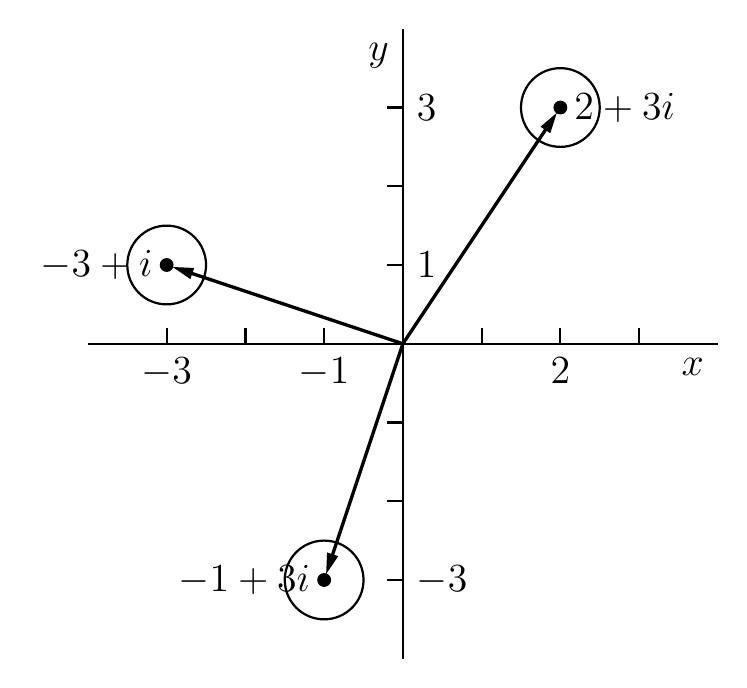
\begin{tikzpicture}[x=1cm, y=1cm, thick]
	\draw (-4, 0) -- (4, 0) node[below left] {$x$};
	\draw (0, -4) -- (0, 4) node[below left] {$y$};
	
	\coordinate (z) at (2, 3);
	\coordinate (z0) at (-3, 1);
	\coordinate (z1) at (-1, -3);
	
	\draw[-tri, shorten >= 2pt, very thick] (0, 0) -- (z);
	\draw[-tri, shorten >= 2pt, very thick] (0, 0) -- (z0);
	\draw[-tri, shorten >= 2pt, very thick] (0, 0) -- (z1);
	
	\fill (z) circle (2.5pt) node[right]{$2 + 3i$};
	\fill (z0) circle (2.5pt) node[left]{$-3+i$};
	\fill (z1) circle (2.5pt) node[left]{$-1 + 3i$};
	
	\foreach \x in {z, z0, z1}{\draw[color=black] (\x) circle (0.5);}
	
	\foreach \x in {-3,-2,-1,1,2,3} {\draw (\x, 0) -- (\x, 0.2);}
	\foreach \y in {-3,-2,-1,1,2,3} {\draw (0, \y) -- (-0.2, \y);}
	
	\foreach \x in {2,-3, -1} {
		\node[below] at (\x, 0) {$\x$};
	}
	\foreach \y in {1,3, -3} {
		\node[right] at (0, \y) {$\y$};
	}
\end{tikzpicture}

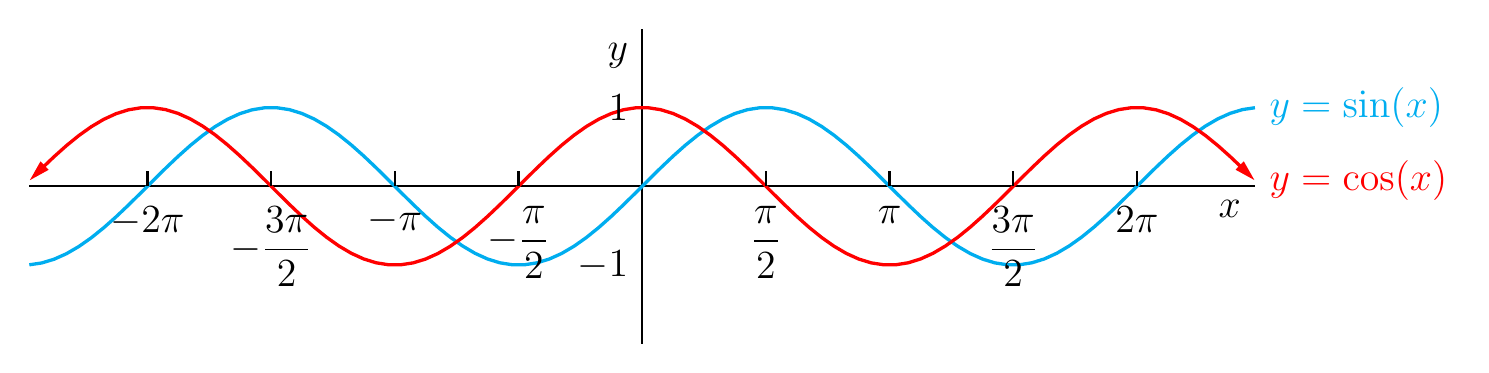
\begin{tikzpicture}[x=1cm, y=1cm, thick]
	\draw (-2*pi-1.5, 0) -- (2*pi+1.5, 0) node[below left] {$x$};
	\draw (0, -2) -- (0, 2) node[below left] {$y$};
	
	

	
	
	\draw[cyan,domain=-2*pi-1.5:2*pi+1.5, samples=100, very thick] plot ({\x}, {sin(deg(\x))}) node[right]{$y = \sin(x)$};
	
	\draw[tri-tri, red,domain=-2*pi-1.5:2*pi+1.5, samples=100, very thick] plot ({\x}, {cos(deg(\x))}) node[right]{$y = \cos(x)$};
	
	\foreach \y in {-1,1} {
		\node[left] at (0, \y) {$\y$};
	}
	\foreach \x/\lbl in {
		-2*pi/$-2\pi$, -1.5*pi/$-\dfrac{3\pi}{2}$, -pi/$-\pi$, -0.5*pi/$-\dfrac{\pi}{2}$,
		0.5*pi/$\dfrac{\pi}{2}$, pi/$\pi$, 1.5*pi/$\dfrac{3\pi}{2}$, 2*pi/$2\pi$
	} {
		\draw (\x, 0) -- (\x, 0.2) node[below, yshift=-8pt] {\lbl};
	}
\end{tikzpicture}

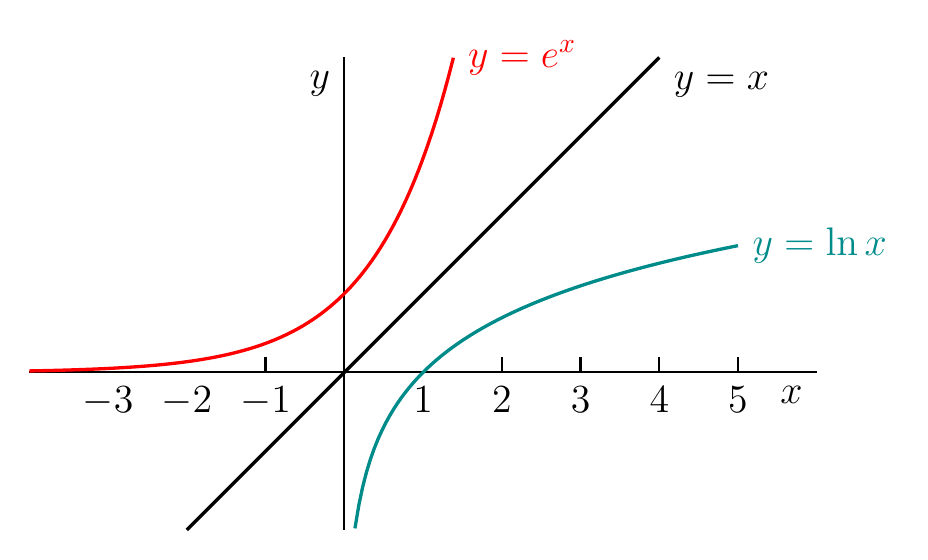
\begin{tikzpicture}[x=1cm, y=1cm, thick]
	\draw (-4, 0) -- (6, 0) node[below left] {$x$};
	\draw (0, -2) -- (0, 4) node[below left] {$y$};
	
	\draw[darkcyan, domain=e^(-2):5, samples=100, very thick] plot ({\x}, {ln(\x)}) node[right]{$y = \ln x$};
	\draw[red,domain=-4:ln(4), samples=100, very thick] plot ({\x}, {e^(\x)}) node[right]{$y = e^x$};
	
	\foreach \x in {-1,2, 3, 4, 5} {\draw (\x, 0) -- (\x, 0.2);}
	\foreach \x in {-3,-2,-1,1,2,3,4,5} {
		\node[below] at (\x, 0) {$\x$};
	}
	\draw[domain=-2:4, samples=2, very thick] plot ({\x}, {\x}) node[below right]{$y=x$};
\end{tikzpicture}


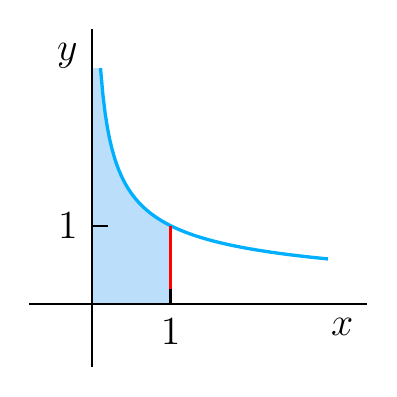
\begin{tikzpicture}[x=1cm, y=1cm, thick]
	
	
	\fill[skyblue] (0, 0) -- (0, 3) -- 
	plot[domain=1/9:1, samples=100] ({\x}, {1/sqrt(\x)}) -- (1,0) -- cycle 
	;
	
	\draw[lightblue, domain=1/9:3, samples=100, very thick] plot ({\x}, {1/sqrt(\x)});
	\draw[red] (1, 0) -- (1, 1);
	\foreach \x in {1} {\draw (\x, 0) -- (\x, 0.2);}
	\foreach \y in {1} {\draw (0, \y) -- (0.2, \y);}
	\foreach \x in {1} {
		\node[below] at (\x, 0) {$\x$};
	}
	\foreach \y in {1} {
		\node[left] at (0, \y) {$\y$};
	}
	
	\draw (-0.8, 0) -- (3.5, 0) node[below left] {$x$};
	\draw (0, -0.8) -- (0, 3.5) node[below left] {$y$};
\end{tikzpicture}

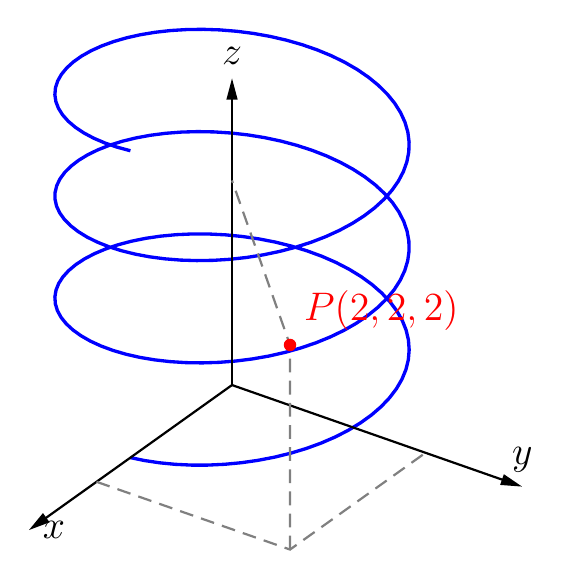
\begin{tikzpicture}[3d view={125}{30}, scale=1.5, thick]
	% 3d view={azimuth}{elevation}
	
	\draw[blue, very thick, domain=0:1080, samples=200, variable=\t]
	plot ({1.5*cos(\t)}, {1.5*sin(\t)}, {\t/360});
	
	% Axes
	\draw[-tri] (0,0,0) -- (3,0,0) node[right] {$x$};
	\draw[-tri] (0,0,0) -- (0,3,0) node[above] {$y$};
	\draw[-tri] (0,0,0) -- (0,0,3) node[above] {$z$};
	
	% Point at (2, 2, 2)

	
	% Projection lines
	\draw[dashed, gray] (2,0,0) -- (2,2,0) -- (0,2,0);
	\draw[dashed, gray] (2,2,0) -- (2,2,2) -- (0,0,2);
	\fill[red] (2,2,2) circle (1.5pt) node[above right] {$P(2,2,2)$};
\end{tikzpicture}

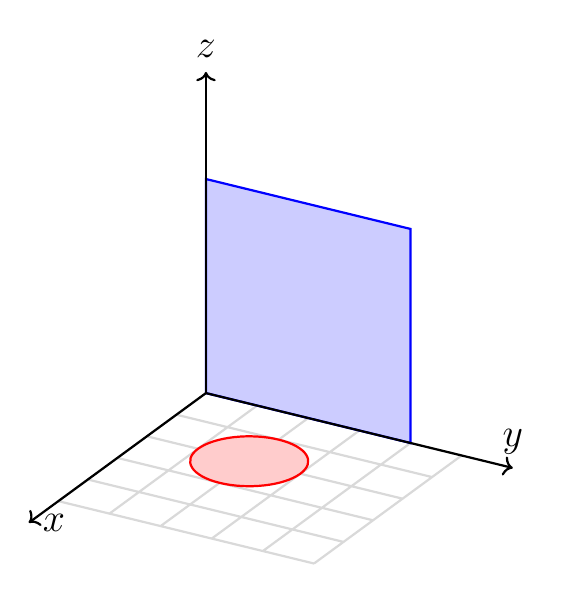
\begin{tikzpicture}[3d view={120}{25}, scale=1.5, thick]
	% Axes
	
	
	% Draw a grid on the xy-plane at z = 0
	\begin{scope}[canvas is xy plane at z=0]
		\draw[gray!30, step=0.5] (0,0) grid (2.5,2.5);
		\draw[red, fill=red!20] (1,1) circle (0.5); % 2D circle placed in 3D
	\end{scope}
	
	% Draw a square on the yz-plane at x = 0
	\begin{scope}[canvas is yz plane at x=0]
		\draw[blue, fill=blue!20] (0,0) rectangle (2,2);
	\end{scope}
	
	\draw[->] (0,0,0) -- (3,0,0) node[right] {$x$};
	\draw[->] (0,0,0) -- (0,3,0) node[above] {$y$};
	\draw[->] (0,0,0) -- (0,0,3) node[above] {$z$};
\end{tikzpicture}

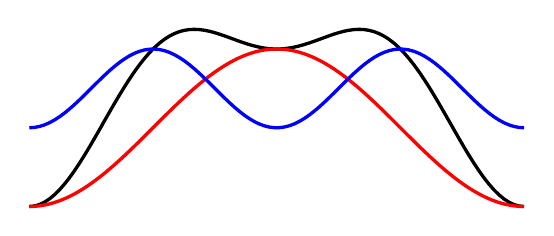
\begin{tikzpicture}[x=1cm, y=1cm, thick, 
	declare function ={
	g(\x) = cos(deg(\x));
	h(\x) = sin(deg(\x))^2;
	f(\x) = g(\x) + h(\x);
	}]
	\draw[domain=-pi:pi, samples=100, very thick] plot ({\x}, {f(\x)});
	
	\draw[red, domain=-pi:pi, samples=100, very thick] plot ({\x}, {g(\x)});
	
	\draw[blue, domain=-pi:pi, samples=100, very thick] plot ({\x}, {h(\x)});
\end{tikzpicture}

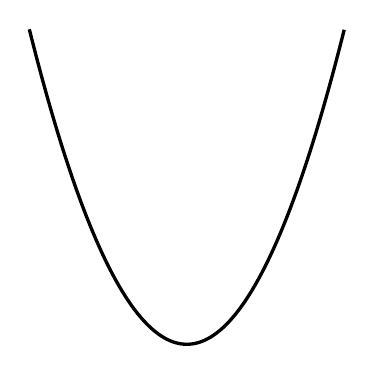
\begin{tikzpicture}[x=1cm, y=1cm, thick]
	\draw[domain=-2:2, samples=100, very thick] plot ({\x}, {(\x)^2});
\end{tikzpicture}

\def\xscale{1}
\def\yscale{1}
\begin{tikzpicture}[x=\xscale cm, y=\yscale cm, thick]
	\draw (-0.5, 0) -- (8, 0) node[below left, xshift=6pt] {$x$};
	\draw (0, -0.5) -- (0, 4) node[below left, yshift=3pt] {$y$};
	
	\node[below left, xshift=2, yshift=2] at (0, 0) {$O$};
	

	\coordinate (z0) at (6,2);
	\coordinate (z) at ($(z0) + (-20:1.3)$);
	
	\draw[color=black, dashed] (z0) circle (1.5);
	
	\draw[-tri, shorten >= 2pt, very thick] (0, 0) --node[pos=0.5, above, sloped]{$z_0$} (z0);
	\draw[-tri, shorten >= 2pt, very thick] (0, 0) --node[pos=0.55, below, sloped]{$z_0 + \Delta z_0$} (z);
	\draw[-tri, shorten >= 2pt, very thick] (z0) -- node[pos=0.5, above, sloped]{$\Delta z$} (z);
	
	\foreach \x in {z0, z}{\fill (\x) circle (2.5pt);}
	
\end{tikzpicture}

\def\xscale{1}
\def\yscale{1}
\begin{tikzpicture}[x=\xscale cm, y=\yscale cm, thick]
	\draw (-2, 0) -- (10, 0) node[below left, xshift=6pt] {$\Delta x$};
	\draw (0, -1) -- (0, 5) node[below left, yshift=3pt] {$\Delta y$};
	\node[below left, xshift=2, yshift=2] at (0, 0) {$(0, 0)$} coordinate (O);
	
	\coordinate (X) at (7, 0);
	\coordinate (Y) at (0, 3);
	
	\foreach \x in {O, X, Y}{\fill (\x) circle (2.5pt);}
	
	\draw[arrow at=0.5] (X) -- (O);
	\draw[arrow at=0.5] (Y) -- (O);
	
	
\end{tikzpicture}

\def\xscale{2.5}
\def\yscale{2.5}
\begin{tikzpicture}[x=\xscale cm, y=\yscale cm, thick]
	\draw (-0.25, 0) -- (2.8, 0) node[below left, xshift=6pt] {$x$};
	\draw (0, -0.25) -- (0, 1.4) node[below left, yshift=3pt] {$y$};
	\node[below left, xshift=2, yshift=2] at (0, 0) {$O$} coordinate (O);
	
	
	\foreach \x in {1,2} {\draw (\x, 0) -- (\x, -0.2/\yscale);}
	\foreach \x in {1,2} {
		\node[below=5pt] at (\x, 0) {$\x$};
	}
	\foreach \y in {1} {\draw (0, \y) -- (-0.2/\xscale, \y);}
	\foreach \y in {1} {
		\node[left] at (0, \y) {$\y$};
	}
	
	\coordinate (A) at (1,1);
	\coordinate (B) at (2, 1);
	\node[above] at (A) {$1+i$};
	\node[above] at (B) {$2+i$};
	
	\foreach \x in {O,A,B}{\fill (\x) circle (2.5pt);}
	
	\draw[arrow at=0.5, very thick] (O) -- (A);
	\draw[arrow at=0.5, very thick] (A) -- (B);
	
\end{tikzpicture}


\def\xscale{1}
\def\yscale{1}
\begin{tikzpicture}[x=\xscale cm, y=\yscale cm, thick]
	\draw (-0.5, 0) -- (8, 0) node[below left, xshift=6pt] {$\tau$};
	\draw (0, -0.5) -- (0, 4) node[below left, yshift=3pt] {$t$};
	\node[below left, xshift=2, yshift=2] at (0, 0) {$O$} coordinate (O);
	
	\coordinate (A) at (1,1);
	\coordinate (B) at (6, 3);
	\foreach \x in {A, B}{\fill (\x) circle (2.5pt);}
	
	\draw (A) to[bend left=10] (B);
	
	\node[below] at (1,0) {$\alpha$};
	\node[below] at (6, 0) {$\beta$};
	
	\node[left] at (0,1) {$a$};
	\node[left] at (0,3) {$b$};
	
	\foreach \x/\y in {1/A, 6/B}{\draw[dashed] (\x, 0) -- (\y);}
	\foreach \x/\y in {1/A, 3/B}{\draw[dashed] (0, \x) -- (\y);}
\end{tikzpicture}


\end{document}